In the 2013 Technical Design Report of the ILC \cite{ILC:TechnicalDesignReport}, the Global Design Effort produced a `value estimate' of 7.8 ILCU (1 ILCU is 1 US Dollar in Jan 2012) with 23 million person hours ($\sim$13,000 person years) of additional labour; This labour is defined as “explicit” labour provided by the collaborating laboratories and institutions, or purchased from industrial firms and is to be distinguished from a company’s `implicit' labour associated with the industrial production of components and contained (implicitly) within the purchase price.  
 
A value estimate is a common form of costing large international projects which are usually built largely from in-kind contribution from participating nation. It has been used by ITER and LHC. This estimate represents the cost of constructing a 500 GeV linear collider averaged over three regional sample sites \textemdash with a variance estimate of 2\% between the three regional sites. It includes a small number of items rated for 1TeV to enable a later upgrade. The value estimate omits a number of items such as pre-construction, taxes, contingency, escalation, spare equipment, beam commissioning, etc. The value estimate has an uncertainty of 25\% (cost premium) and a more accurate estimate will be calculated when the host site is confirmed and the international governance and in-kind contribution is agreed upon.
 
The value estimate of \$7.8 billion is dominated by the super conducting radio frequency (SCRF) components and related LINAC systems, together with the conventional facilities and siting (CFS). These two elements account for 73\% of the total. The main LINAC itself corresponds to 67\% of the total project. Installation and laboratory management are the biggest single elements. The CFS design and costs can be broken down into three main areas: civil construction, including underground and surface structures, shafts and access tunnels; electrical systems (AC power distribution etc.); and mechanical systems (water cooling and air handling etc.).
 
\begin{figure}[!htb]
\centering
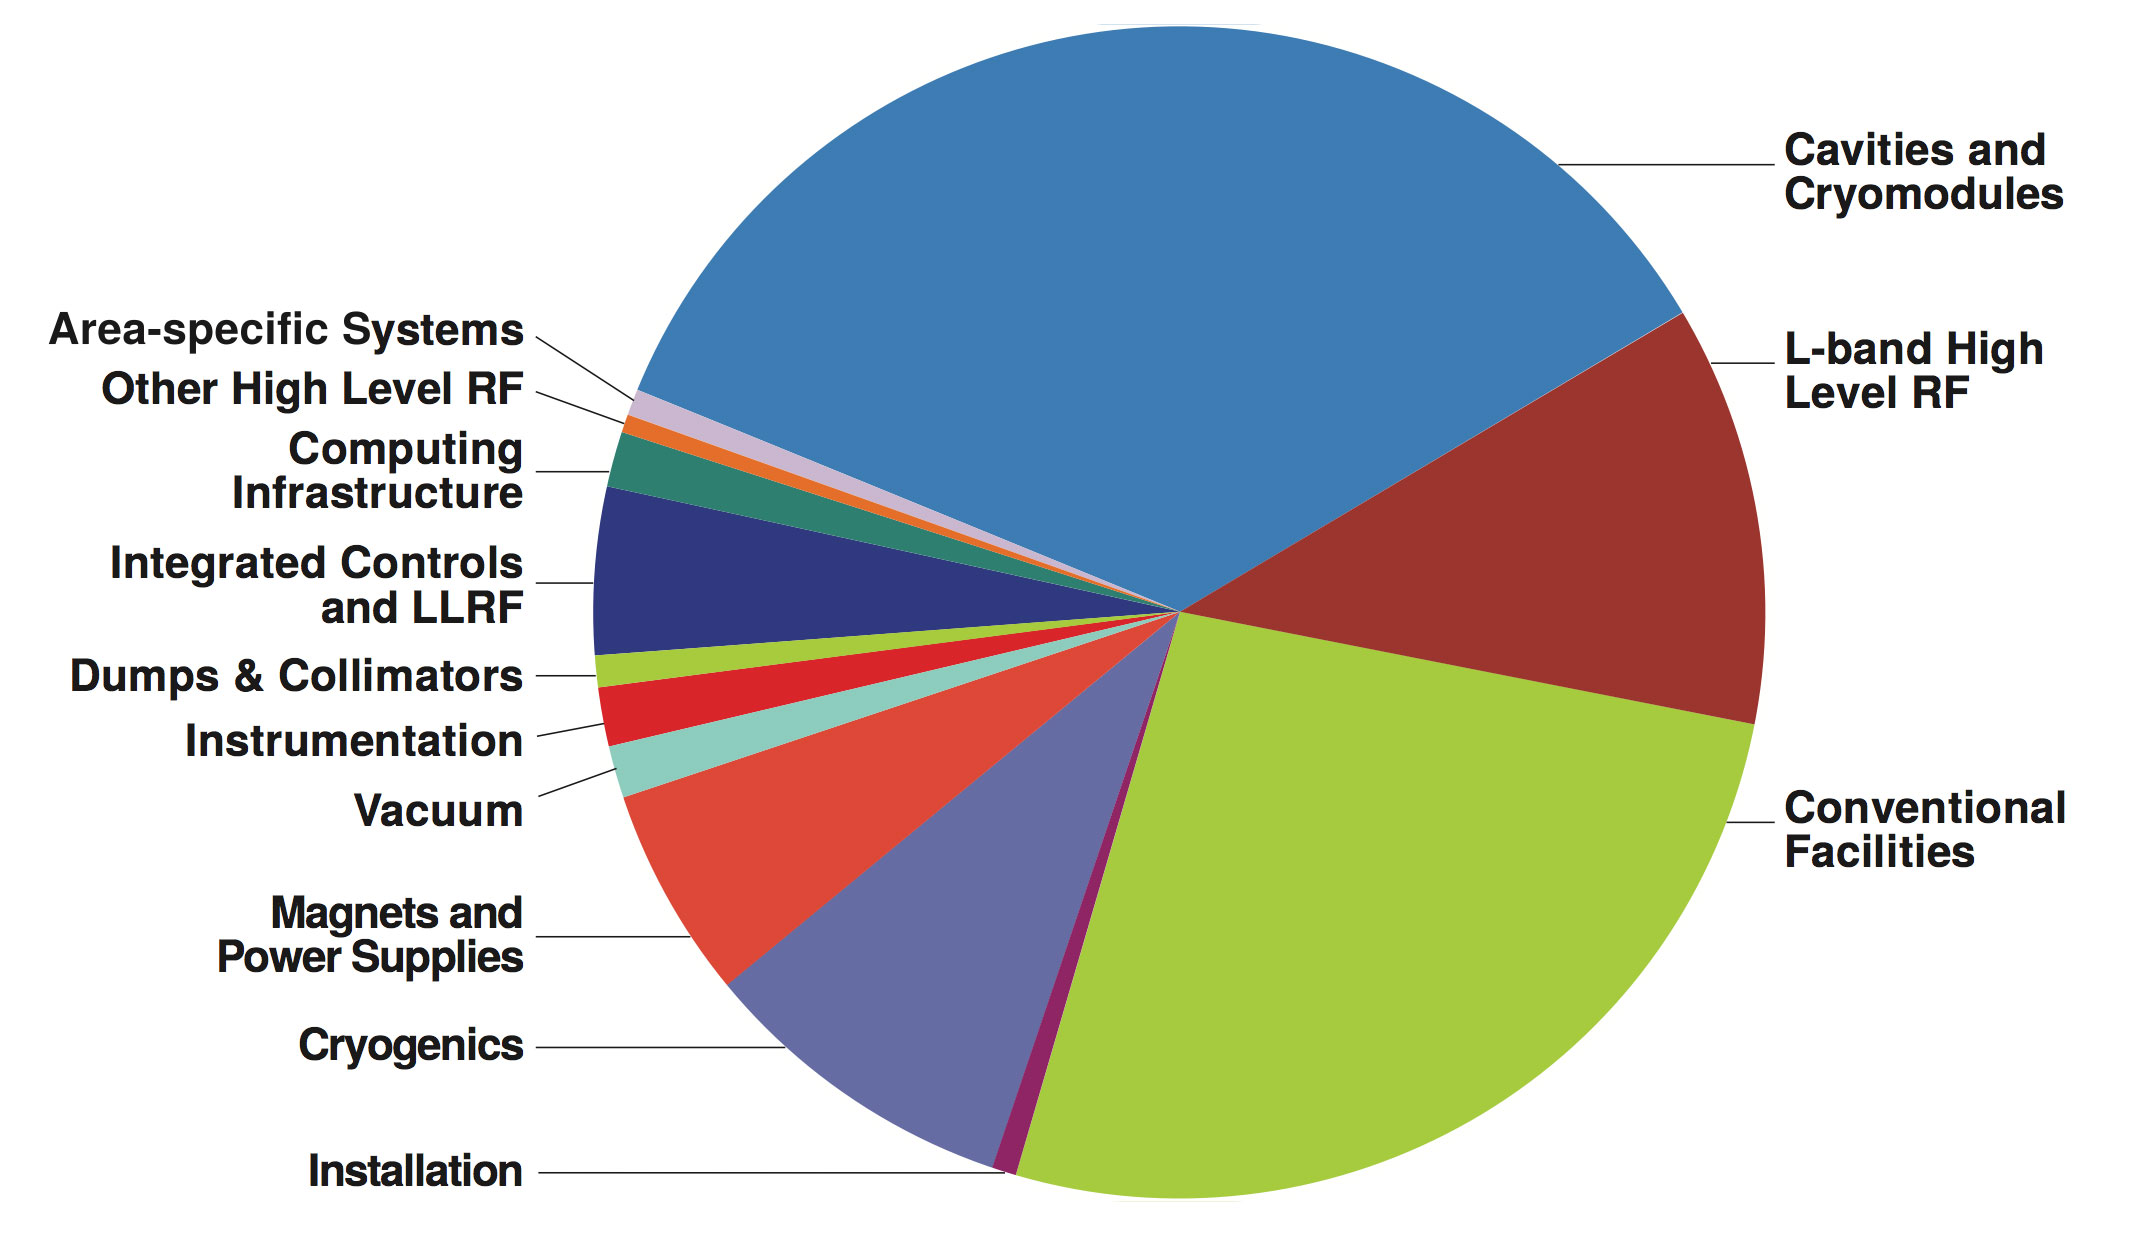
\includegraphics[width=1\textwidth,natwidth=2132,natheight=1246]{ILC_Cost.jpg}
\caption{Sub-system value breakdown \cite{ILC:TechnicalDesignReport}}
\end{figure}
 
The host site geology will determine the most cost-effective tunnelling method approach, while topography can influence the surface structures, access tunnels and shafts. All of these factors can shift the balance of the cost-optimisation and influence the accelerator design. As a result, the final machine will be influenced by the choice of site. In the absence of a definitive site for the ILC, evaluations of different characteristic sites were made. \cite{ILC:TechnicalDesignReport}
 
\subsubsection{Detector costs}

The SiD detector’s cost estimate is a construction cost estimate which excludes R\&D, commissioning, operating costs, or physicist salaries. The SiD cost is \$315 million for M\&S, 316 thousand person-hours engineering, 904 thousand person-hours technical, and 51 thousand person-hours administrative labour. The estimated M\&S contingency, reflecting uncertainty in unit costs and some estimate of the maturity of this study, is \$127 million.

The cost of the ILD detector will depend on the option chosen (two options for the vertex detector, which is a multiple layer silicon pixel sensor measuring the position of charged particles, are that it will either consist of 3 double layers or 5 single layers.) and varies between \$350 and \$440 million. This cost does not include labour, or any contingency.
 
\subsubsection{Cost Growth}

Cost growth has been a very common problem for large science projects. For example, the largest such project, the International Space Station, experienced dramatic cost growth throughout the construction, beginning with documented doubling of the construction cost and followed by continuing cost escalation. The reasons are manyfold, but some of them present important lessons for us, like cost growth due to an evolving design, lack of sufficient mechanisms to control cost growth, etc. So it is not a complete surprise that a recently finished design review of ITER, a major fusion experiment to be built in Cadarache, France, is forecasting a delay of 1-3 years in its completion date and a roughly 25-30\% increase in its 5-billion (US\$7.8-billion) construction cost. Closer to home, the Large Hadron Collider (LHC) also experienced both cost growth and subsequent delays in schedule. The project was originally approved in 1995 for a budget of 2.6 billion Swiss Francs, plus 210 million Swiss Francs for the experiments. The project underwent a major review in 2001, resulting in an increased budget and a delay in the start date from 2005 to 2007. By the time of actual commissioning in 2010, the costs had grown well beyond the original budgets. Problems with magnets were a major contributor, but underestimating the costs when the project was proposed and approved was also a big factor. \cite{ILC:CostMegaprojects}
  
\subsubsection{Construction Cost}

Earlier reports on governance generally favoured a regional approach to funding, e.g. the host region providing 50\% of the overall cost and the non-host regions 25\% each. Developments since the date of these reports increasingly call into question the viability of such models. The rapid industrialisation of in particular China and India and their increasing expenditures on science have changed the face of science in Asia. Japan no longer dominates the scene, although it is still by far the strongest participant in particle physics. Still, both India and China have greatly increased activity. Since, unlike the situation in Europe, there is no strong coordinating institution similar to the EU, it is difficult to see how an Asian contribution to the ILC could be apportioned without complex multilateral negotiations in an undefined forum. Similarly, the relative commitment of the US to particle physics has declined to the extent that it does not seem likely that the Department of Energy would be willing to invest 25\% of the ILC cost in a facility overseas.
 
The 50:25:25 model of regional contributions is more or less a GDP-related model, similar to that used by CERN, though it uses Net National Income (NNI) rather than GDP. A model for the ILC based on that used by CERN could be considered; it has a saturation feature that no one country can contribute more that 25\% of the total CERN budget. Unfortunately as remarked above, it seems unlikely that the US would be willing to contribute 25\% of the project cost, which is the amount that its GDP would dictate under the CERN-like arrangement.
 
All models must include a substantial `host premium' by which the host pays a significantly larger share of the project than would otherwise be expected. This takes into account the very substantial economic benefits which the host area will attain. The size of such a premium should not be fixed to an arbitrary amount, such as 50\%, but instead should be agreed between the major partners at the start of the project.

Concluding that the ILC funding model should be based on a substantial host premium together with a `share model' in which participants contribute an agreed share of the project not just proportional to GDP or other measures of economic wealth.
 
\subsubsection{Running Cost}

The ICFA guidelines in regard to running costs have been modified to permit operating costs to be shared among the project participants. They say it is important not to double count the benefits of hosting, leading to a premium in both construction and running, unless this is really justified by the economic analysis.

The ICFA recommends that running costs should be evaluated at the time of setting up the organisation and a suitable algorithm agreed to. A commonly chosen algorithm is that running costs should be distributed roughly proportional to capital contributions.
 
\subsubsection{Decommissioning Cost}

It will be the responsibility of the state that provided the particular Work Breakdown Structure (WBS) item to decommission it; the host should have enduring responsibility, including if necessary returning the site to the condition before the project was constructed.